\documentclass{article}
\usepackage{listings}
\usepackage{verbatim}
\lstset{
    frame=single,
    breaklines=true
}
\usepackage{geometry}
\geometry{margin=1in}		%set margins

\usepackage{graphicx}		%need for images
\usepackage{float}			%need for arranging graphics and tables


\title{ECG 782 HW 2}
\date{2015-10-7}
\author{Carlo Lopez-Tello}

\begin{comment}

how to paste code

\lstinputlisting[language=Octave]{Q1/histEqualize.m}

how to paste image

\begin{figure}[H]
	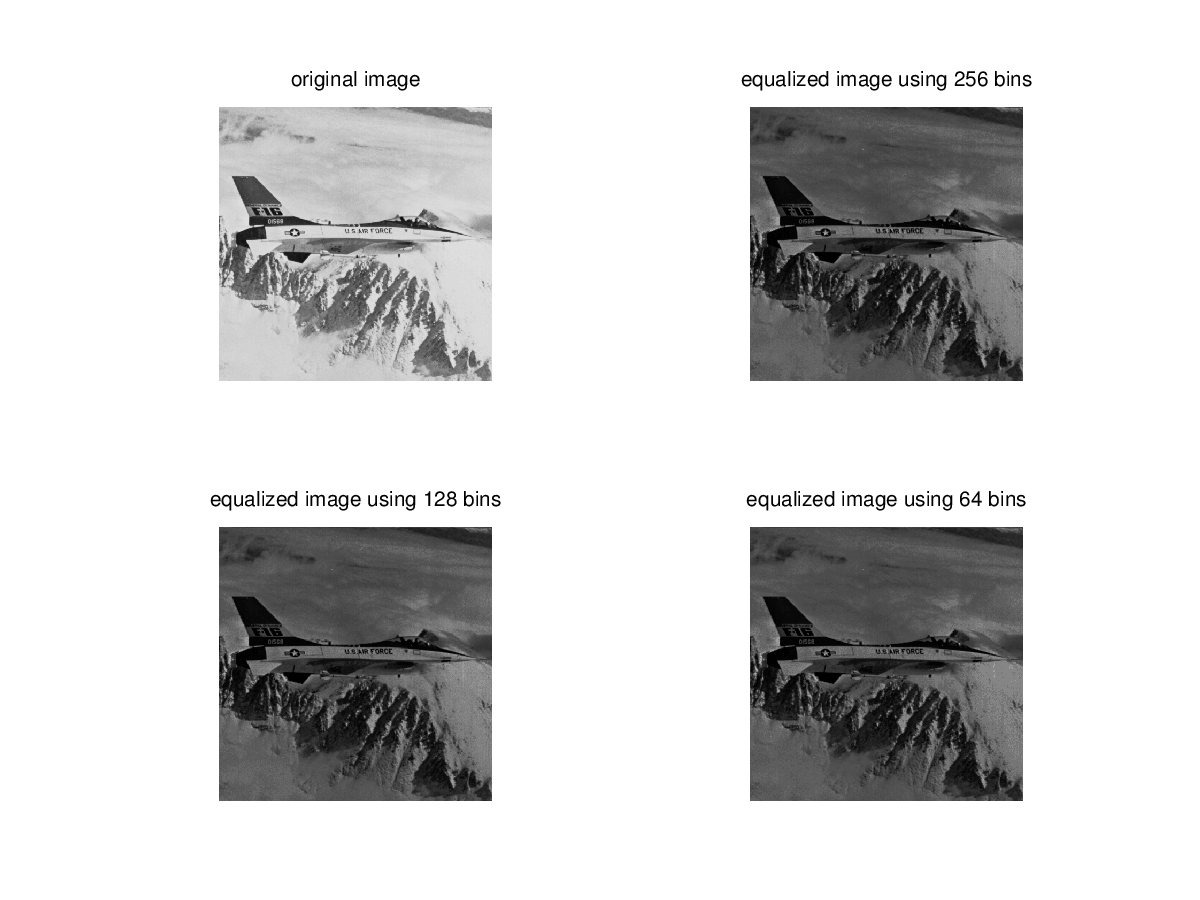
\includegraphics[width=\linewidth]{Q1/outputImages.png}
	\caption{equalized images}
\end{figure}

how to start newpage

\newpage

how to make table

\begin{table}[H]
	\centering
	\begin{tabular}{ c | c | c }
		filter & MSE & PSNR \\
		none & 72.0 & 29.6 \\
		3x3 mean filter & 32.9 & 33.0 \\
		5x5 mean filter & 36.7 & 32.5 \\
		3x3 median filter & 37.2 & 32.4 \\
		5x5 median filter & 36.2 & 32.5 \\
	\end{tabular}
	\caption{SNR and PSNR after filtering the noisy image}
\end{table}
	

\end{comment}
\begin{document}
\maketitle
	\newpage
	\section{Problem 4.4: Features of cosine}
	\[f(t) = cos(2\pi nt)\]
	The period of \(f(t)\) is \(T=\frac{2\pi}{2\pi n}=\frac{1}{n}\).
	\newline
	The frequency is \(f=\frac{1}{T}=n\).
	\newline
	The Fourier transform of \(f(t)\), \(F(f)\), will look like two deltas, one positive at \(f=n\) and one negative at \(f = -n\). If \(f(t)\) is sampled at a higher sampling frequency than \(fs>2n\) then there will be copies of \(F(f)\) every \(fs\). The copies will be far enough apart that they will not interfere with one another. 
	If \(f(t)\) is sampled at \(fs=2n\) the copies will be too close and cancel each other out.
	If \(f(t)\) is sampled at \(fs<2n\) the copies will be too close and interfere with each other. It will cause the sampled version of \(f(t)\) to have more frequency components. The extra frequency components will be at \(fs-n\) or \(fs-n\) depending on \(fs\).
	
	\begin{figure}[H]
		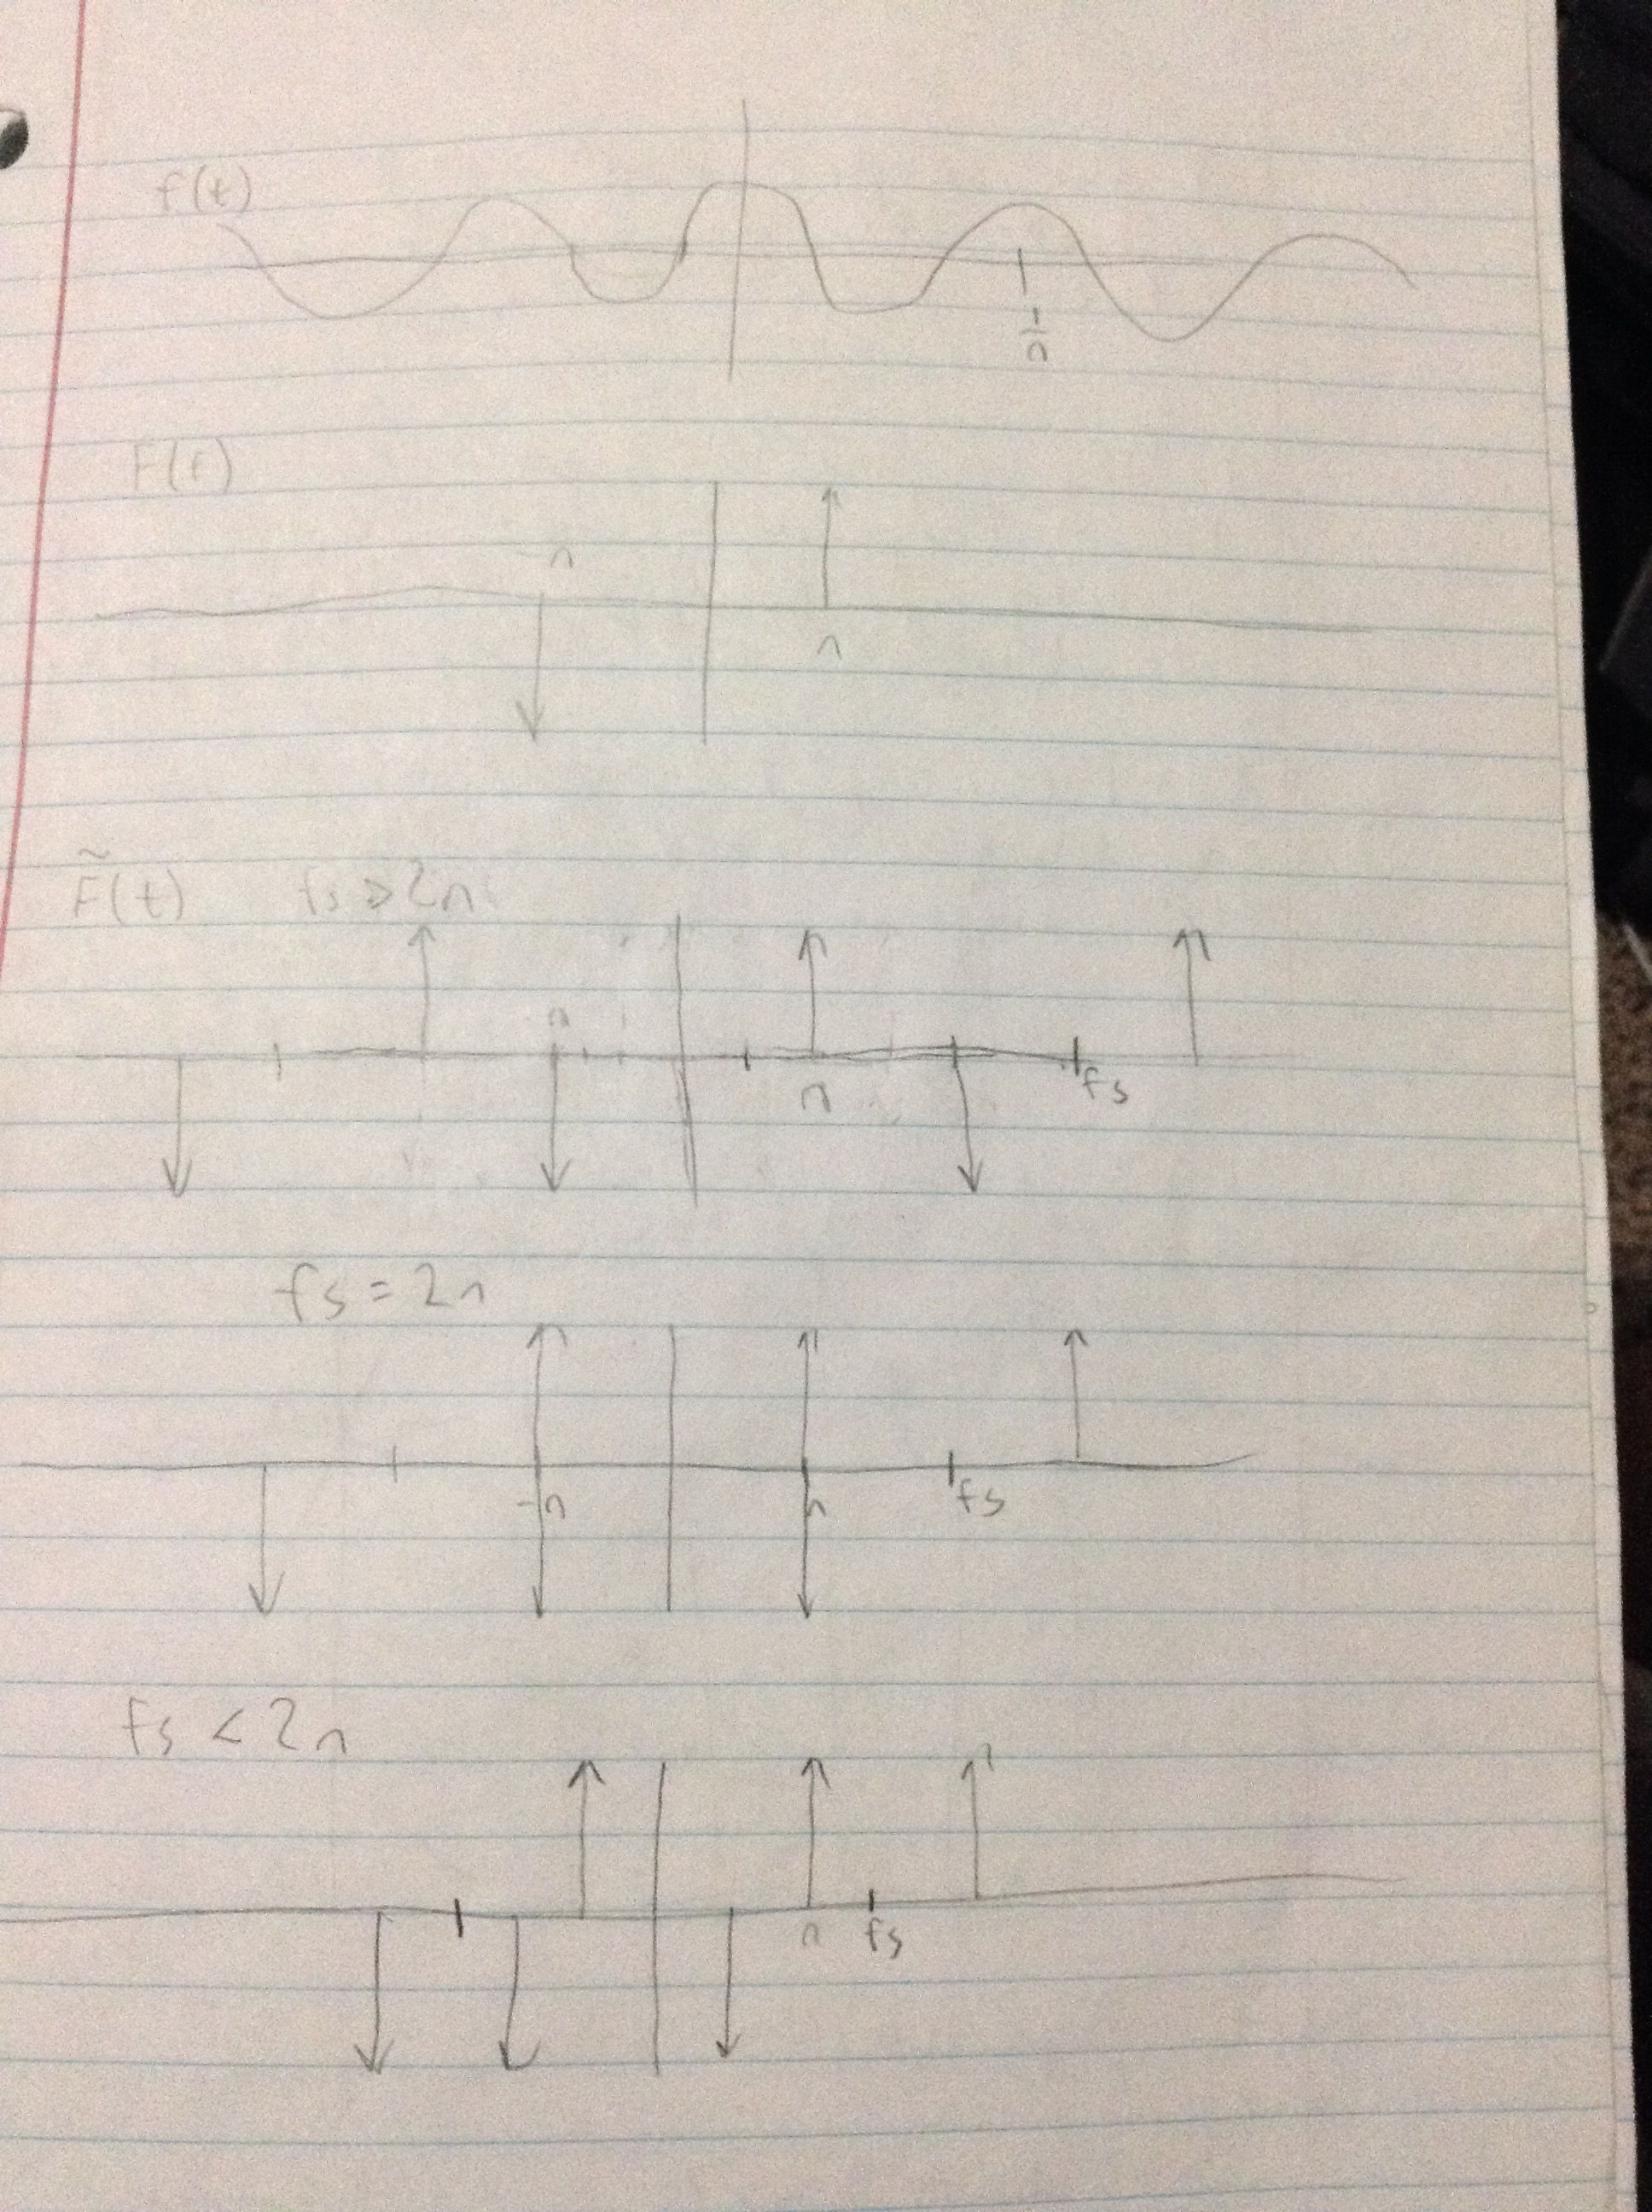
\includegraphics[width=\linewidth]{fig1.JPG}
	\end{figure}
	
	\newpage
	\section{Problem 4.12: Sampling of checkerboard}
	The period of the checkerboard image is \(T = 1mm\). This implies that the image should be sampled at a rate \(fs > \frac{2}{1mm}\).
	\begin{figure}[H]
		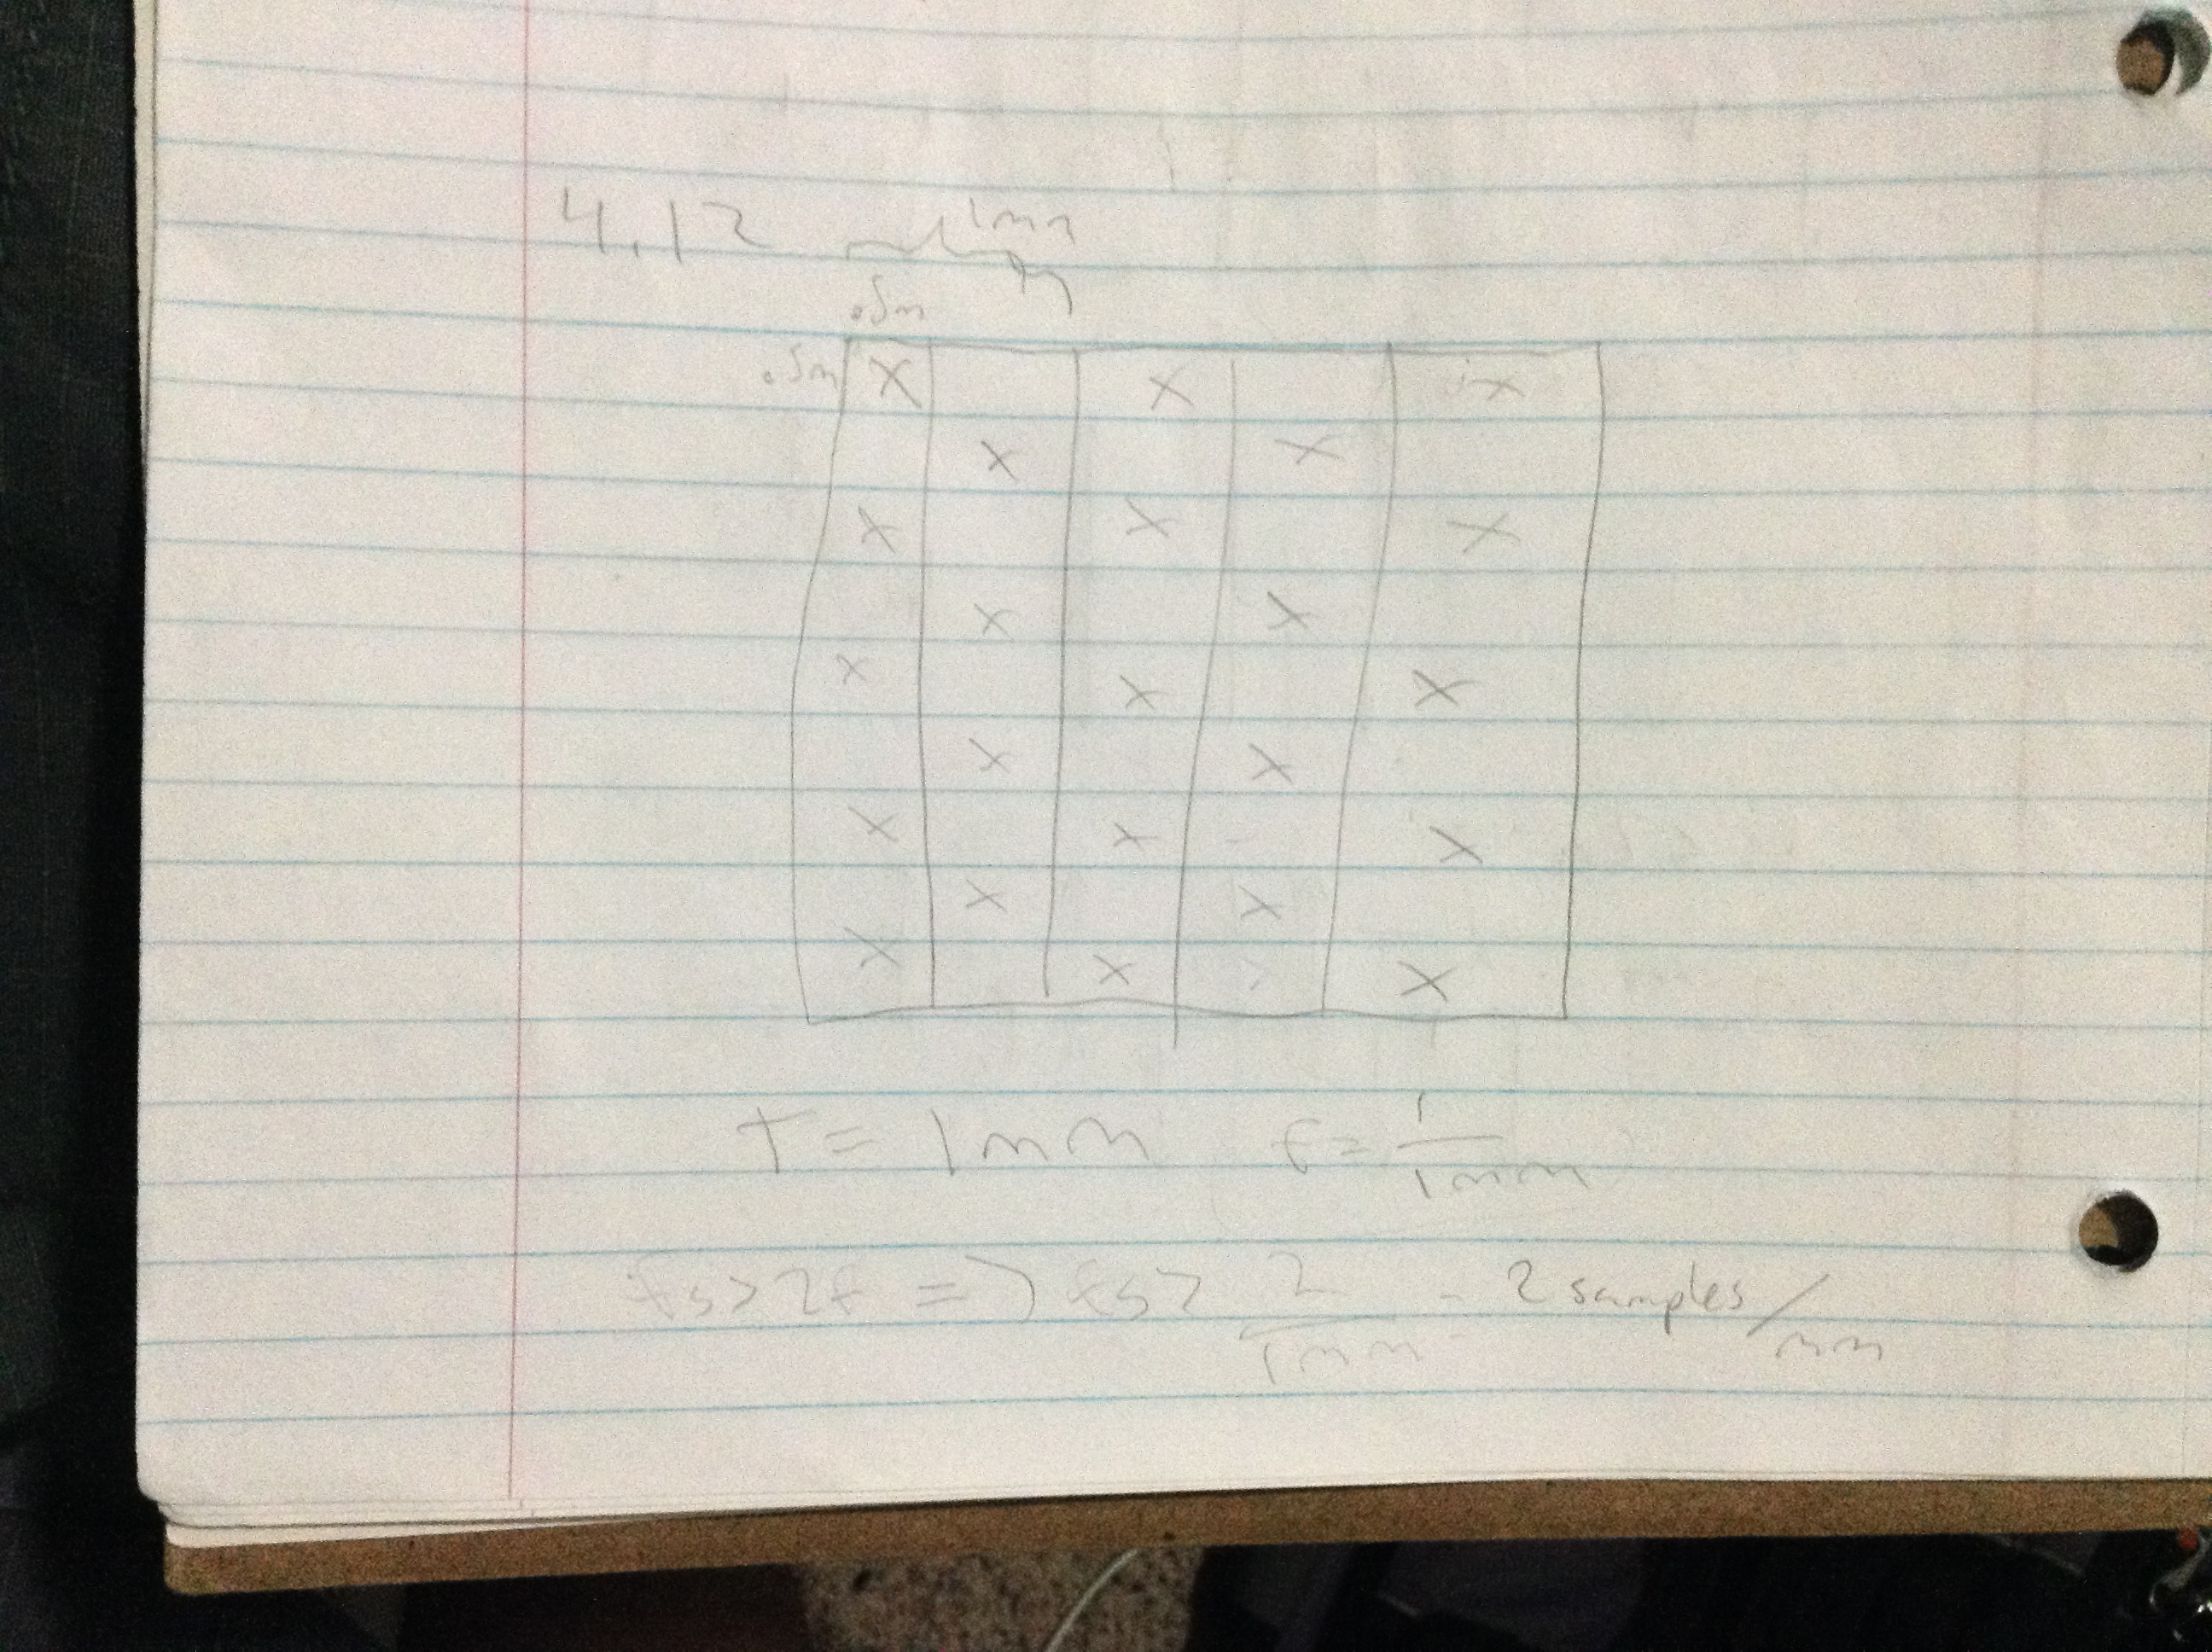
\includegraphics[width=\linewidth]{fig2.JPG}
	\end{figure}
	
	\newpage
	\section{Problem 4.32: What is the form of the spatial domain Gaussian high pass filter}
	A high pass filter can be made using a low pass.
	\[H_{HP} = 1 - H_{LP}\]
	A Gaussian low pass filter has the following form
	\[H_{LP} = e^{-\frac{\mu^2 + v^2}{2\sigma^2}}\]
	therefore
	\[H_{HP} = 1 - e^{-\frac{\mu^2 + v^2}{2\sigma^2}}\]
	we can apply the inverse Fourier transform to get the spatial domain version
	\[h_{HP} = \delta(t,z) - 2\pi\sigma^2 e^{-2\pi^2\sigma^2(t^2 - z^2)}\]
	
	\newpage
	\section{Problem 4.39: Applying high frequency emphasis and histogram equalization}
	The order of operations matters, because histogram equalization is a non linear operation. Therefore, the results will differ depending on which operation is applied first.
	High frequency emphasis should be applied first, since it reduces image contrast. If one were to apply histogram equalization first it would most likely be undone by high frequency emphasis.
	
	\newpage
	\section{Problem 4.43: Cleaning up images}
	1.The best way to remove bright spots would be median filtering.
	\newline
	2.To sharpen an image one should do high frequency filtering and add the edges to the original image.
	\newline
	3.To improve contrast one can apply histogram equalization or gamma correction.
	\newline
	4.If the average intensities vary between images one should first find the desired average intensity \(I_{av}\). Then one can find the difference between the average intensity of an image and the desired intensity \(I_{df} = I_{av}-I_{im}\). To adjust the intensity of a specific image all on has to do is add the difference \(I_{df}\)to every pixel in the image. This procedure works because if one adds a constant to every pixel the average of all the pixels increases by that constant.
	
	\newpage
	\section{Problem 6: Filtering in spacial domain}
	\subsection{Image smoothing}
	\begin{figure}[H]
		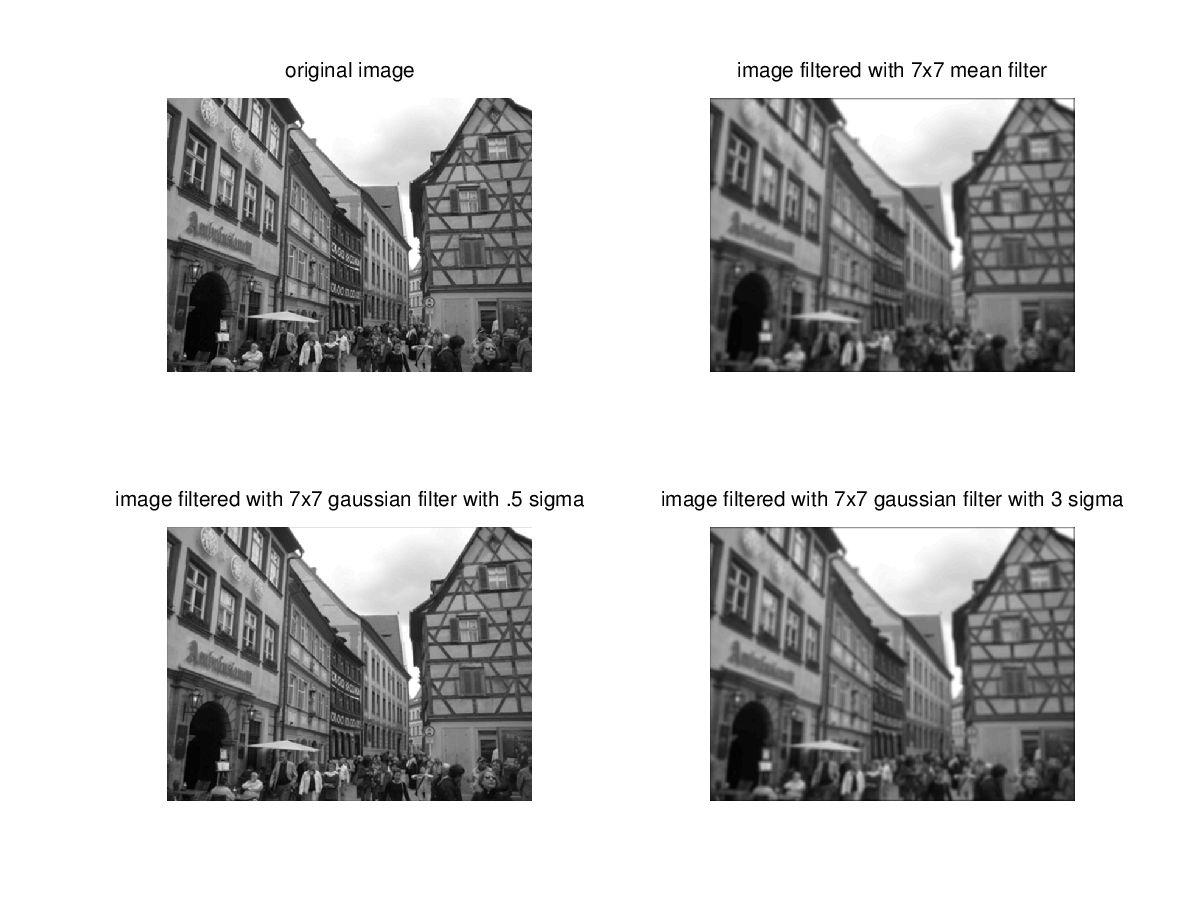
\includegraphics[width=\linewidth]{Q6/partA.png}
	\end{figure}
	The mean filter produces the blurriest image followed by the wider Gaussian filter.
	\subsection{Edge enhancement}
	\begin{figure}[H]
		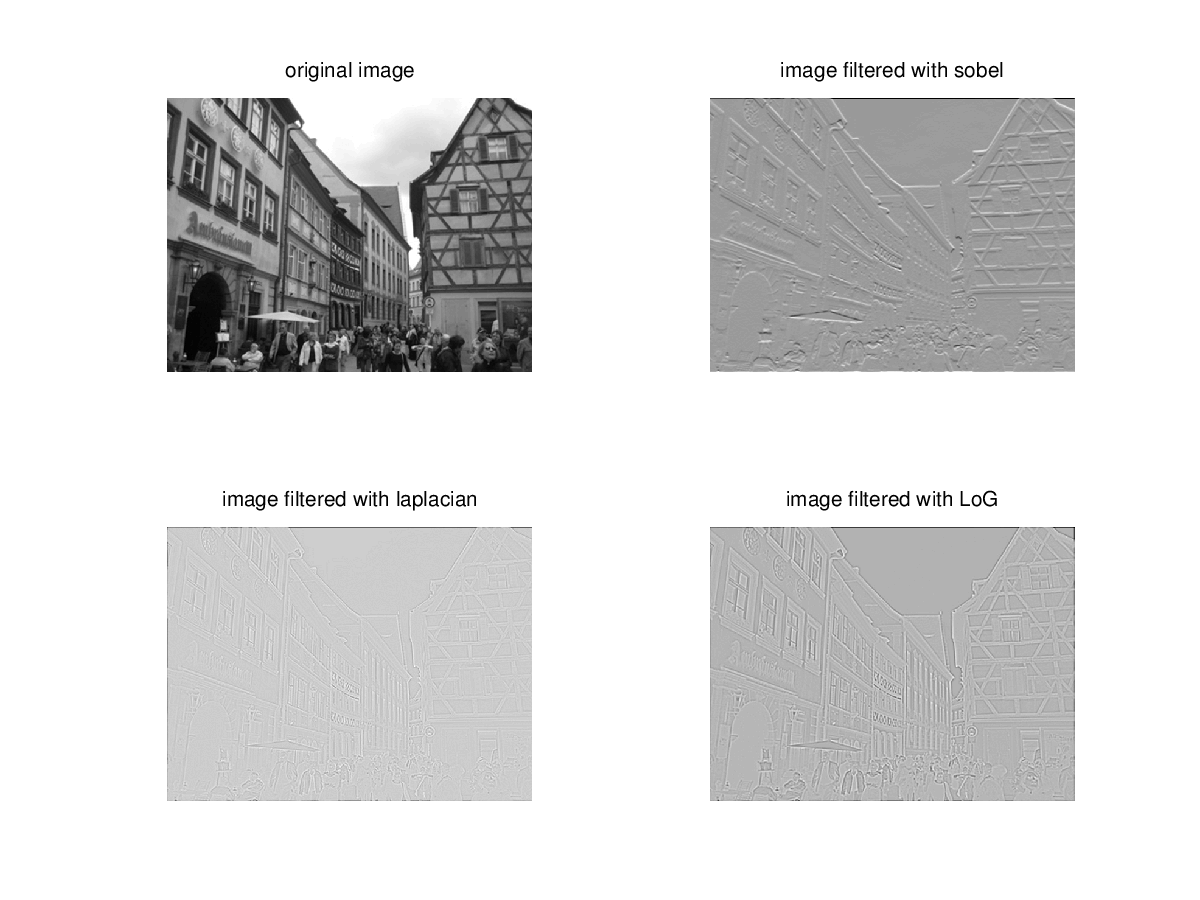
\includegraphics[width=\linewidth]{Q6/partB1.png}
		\caption{output of filters}
	\end{figure}
	
	\begin{figure}[H]
		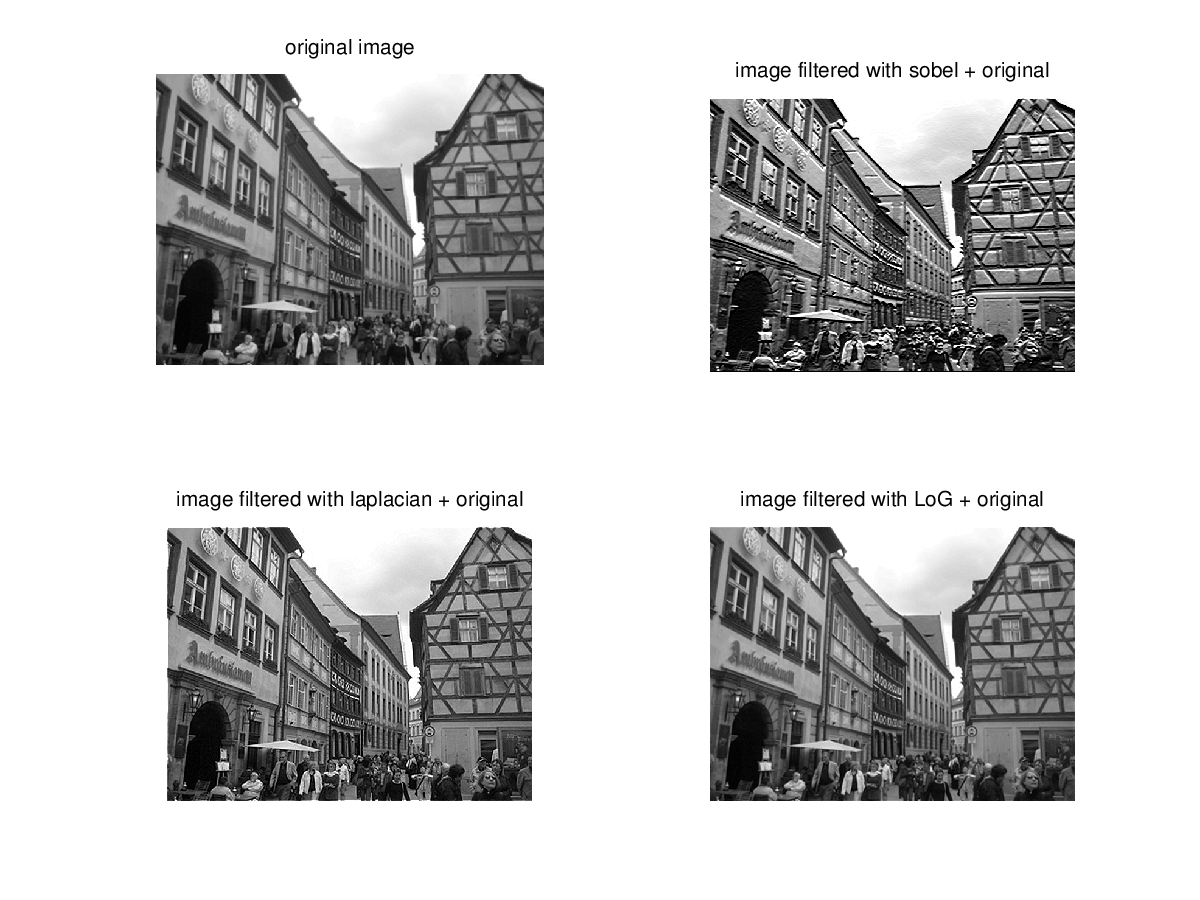
\includegraphics[width=\linewidth]{Q6/partB2.png}
		\caption{enhanced images}
	\end{figure}
	The sobel filter produced the thickest edges, but distorted the image. The laplacian accentuated the edges without distorting the image too much. The LoG sharpened the image without distorting it.
	
	\newpage
	\section{Problem 7: Filtering in frequency domain}
	\subsection{Plot the Fourier transform of 'city.jpg'}
	\begin{figure}[H]
		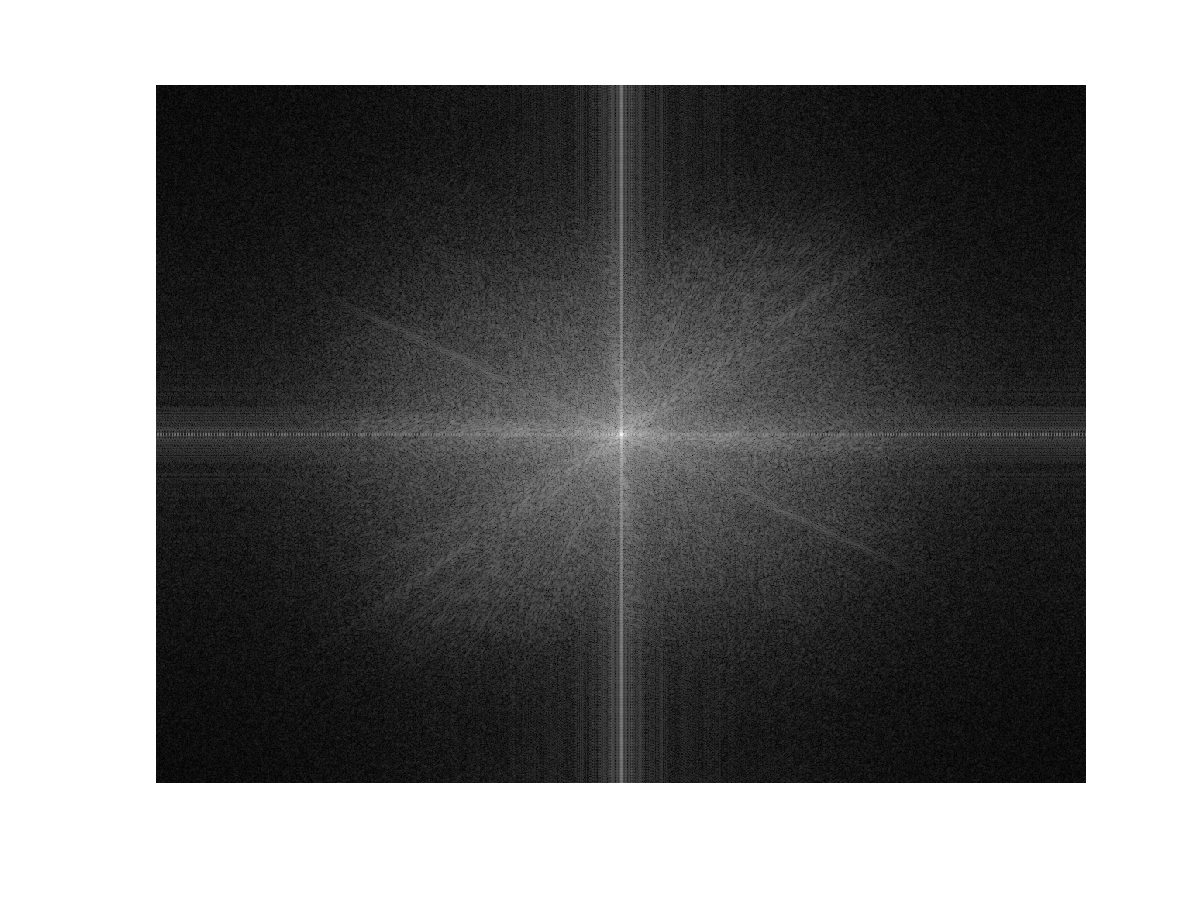
\includegraphics[width=\linewidth]{Q7/partA.png}
		\caption{Fourier transform of 'city.jpg'}
	\end{figure}
	
	\subsection{Comparison between freq domain and spatial domain filtering for smoothing}
	
	\begin{figure}[H]
		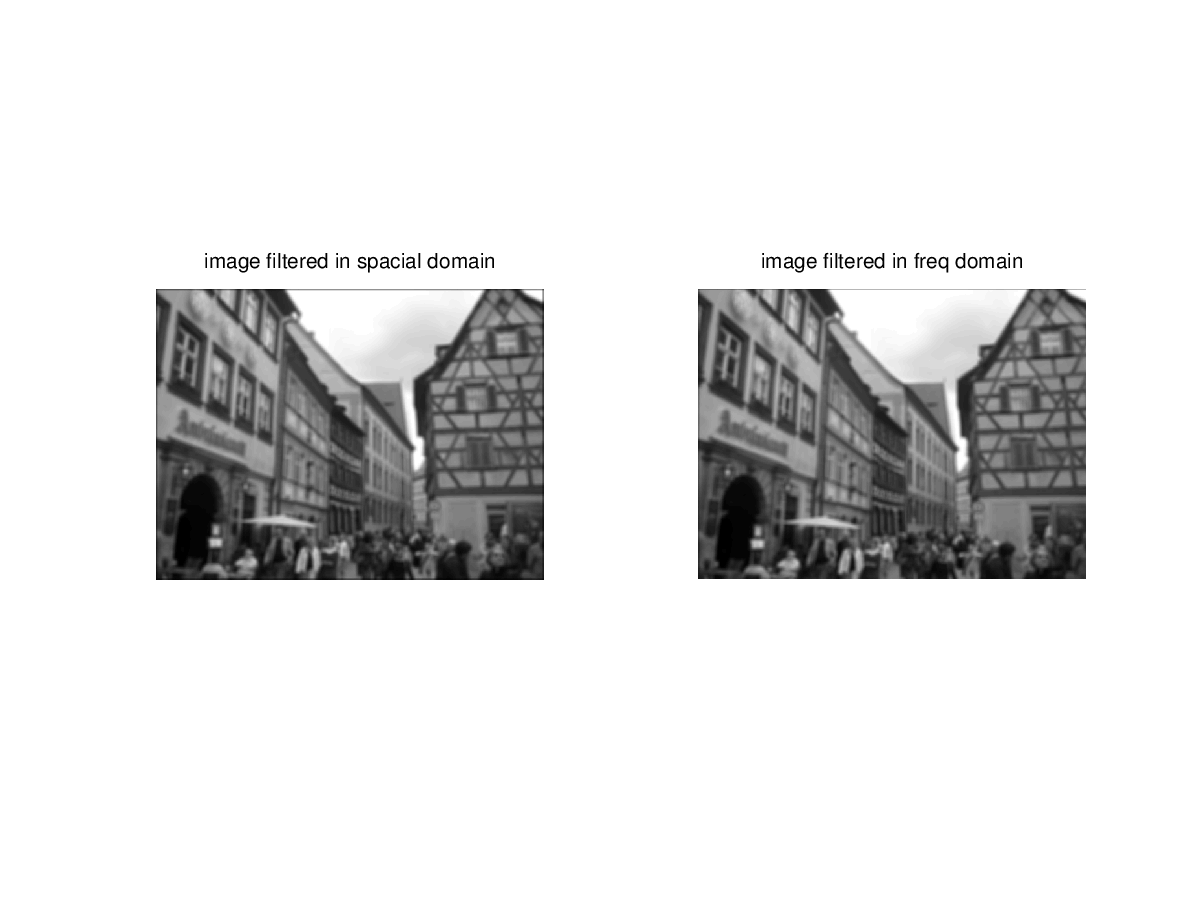
\includegraphics[width=\linewidth]{Q7/partB1.png}
		\caption{image filtered with 7x7 mean filter}
	\end{figure}
	\begin{figure}[H]
		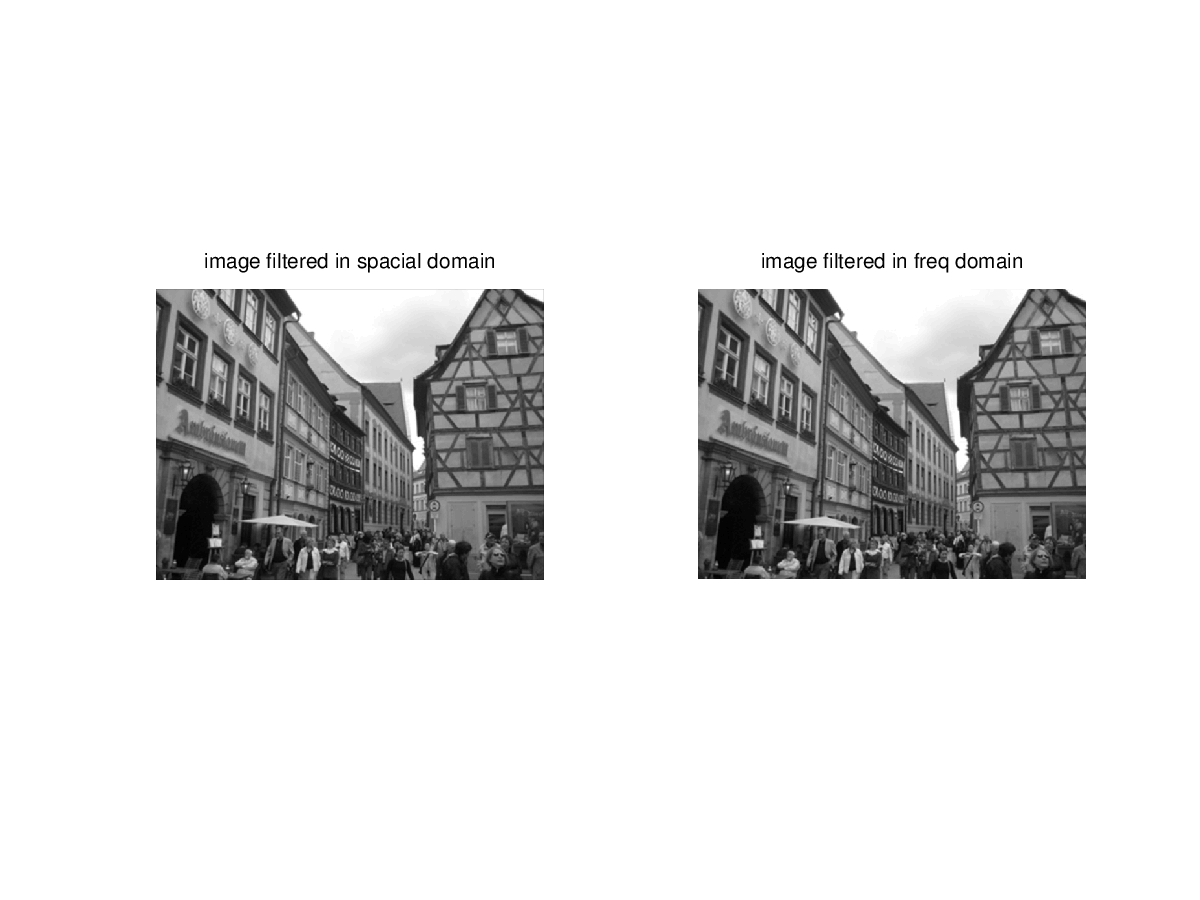
\includegraphics[width=\linewidth]{Q7/partB2.png}
		\caption{image filtered with 3x3, .5 sigma Gaussian filter}
	\end{figure}
	\begin{figure}[H]
		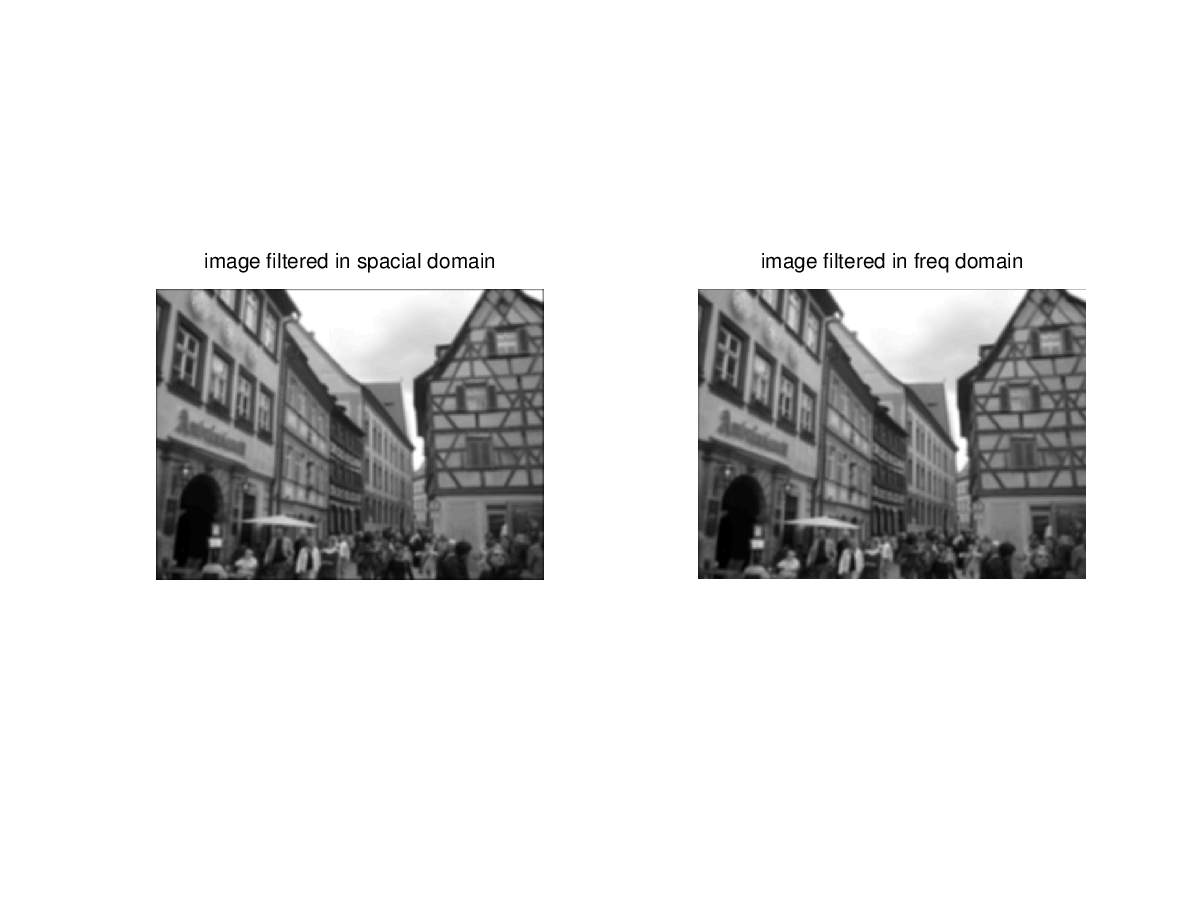
\includegraphics[width=\linewidth]{Q7/partB3.png}
		\caption{image filtered with 3x3, 3 sigma Gaussian filter}
	\end{figure}
	
	There is a significant decrease of performance (5 to 10 times slower) when filtering in the frequency domain.
	\begin{table}[H]
		\centering
		\begin{tabular}{ c | c | c }
			filter & time for spacial dom & time for freq dom \\
			mean filter & .016 & .157 \\
			.5 sigma Gaussian filter & .033 & .197 \\
			3 sigma Gaussian filter & .038 & .157 \\
		\end{tabular}
		\caption{time comparison for filtering in space vs freq domains}
	\end{table}
	
	\subsection{Comparison between freq domain and spatial domain filtering for edge enhancement}
	
	\begin{figure}[H]
		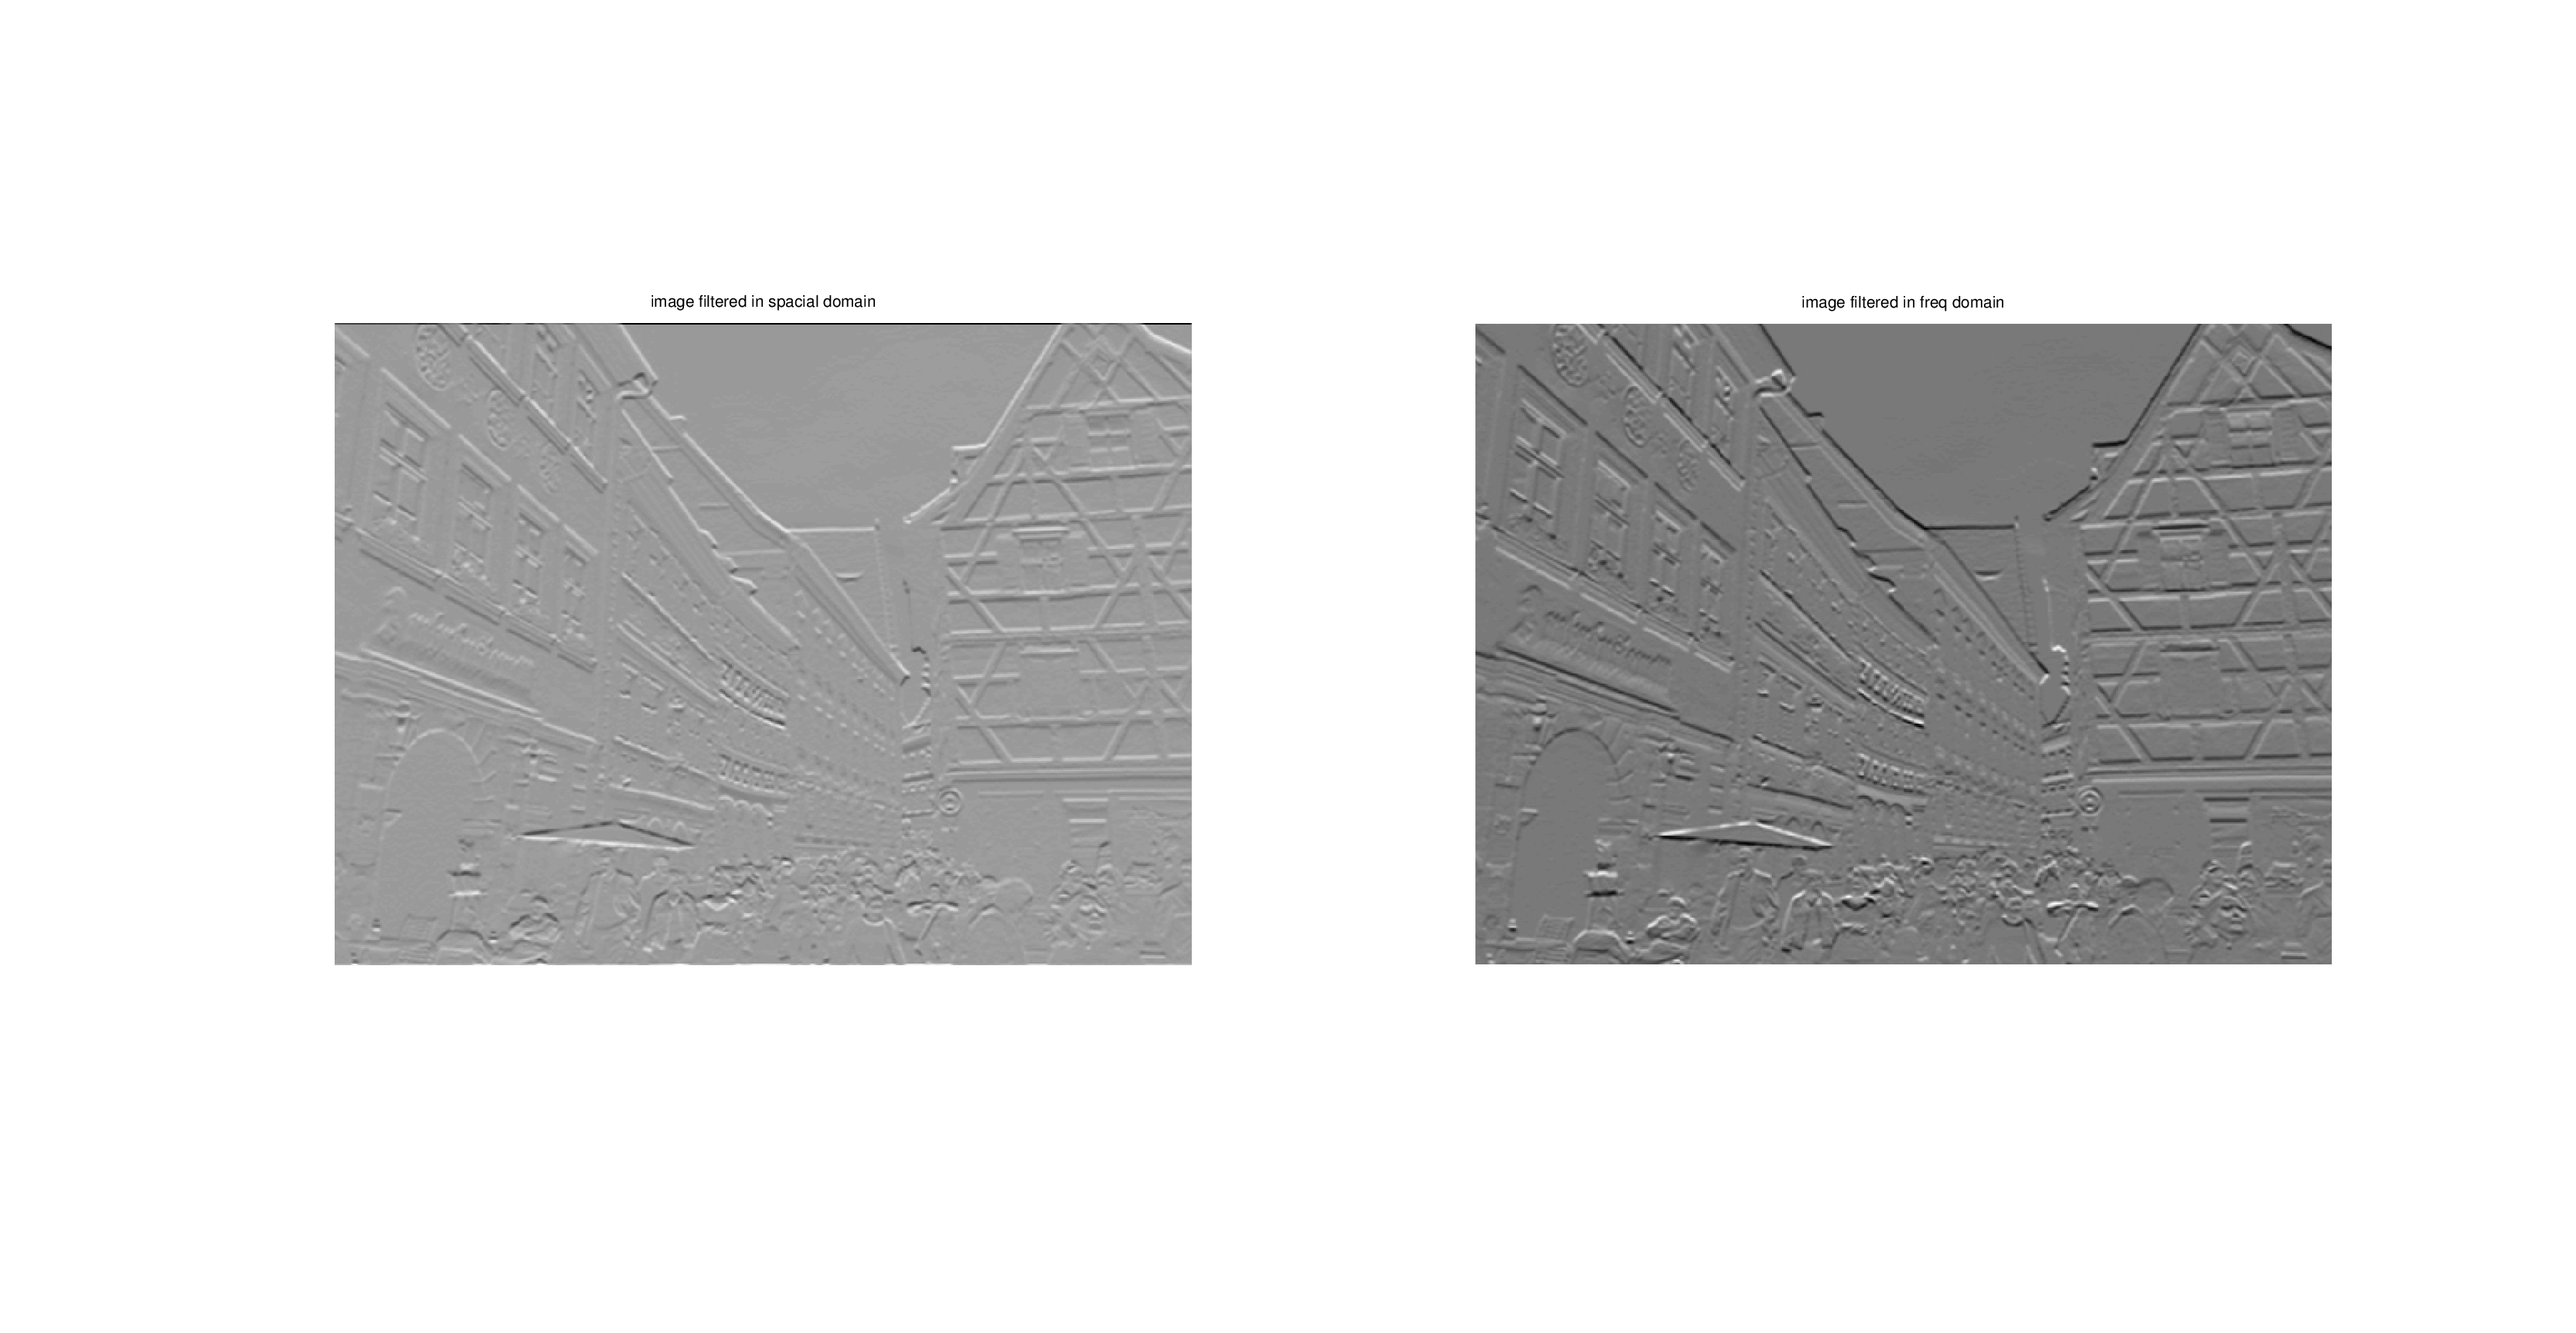
\includegraphics[width=\linewidth]{Q7/partC1.png}
		\caption{image filtered with sobel filter}
	\end{figure}
	
	\begin{figure}[H]
		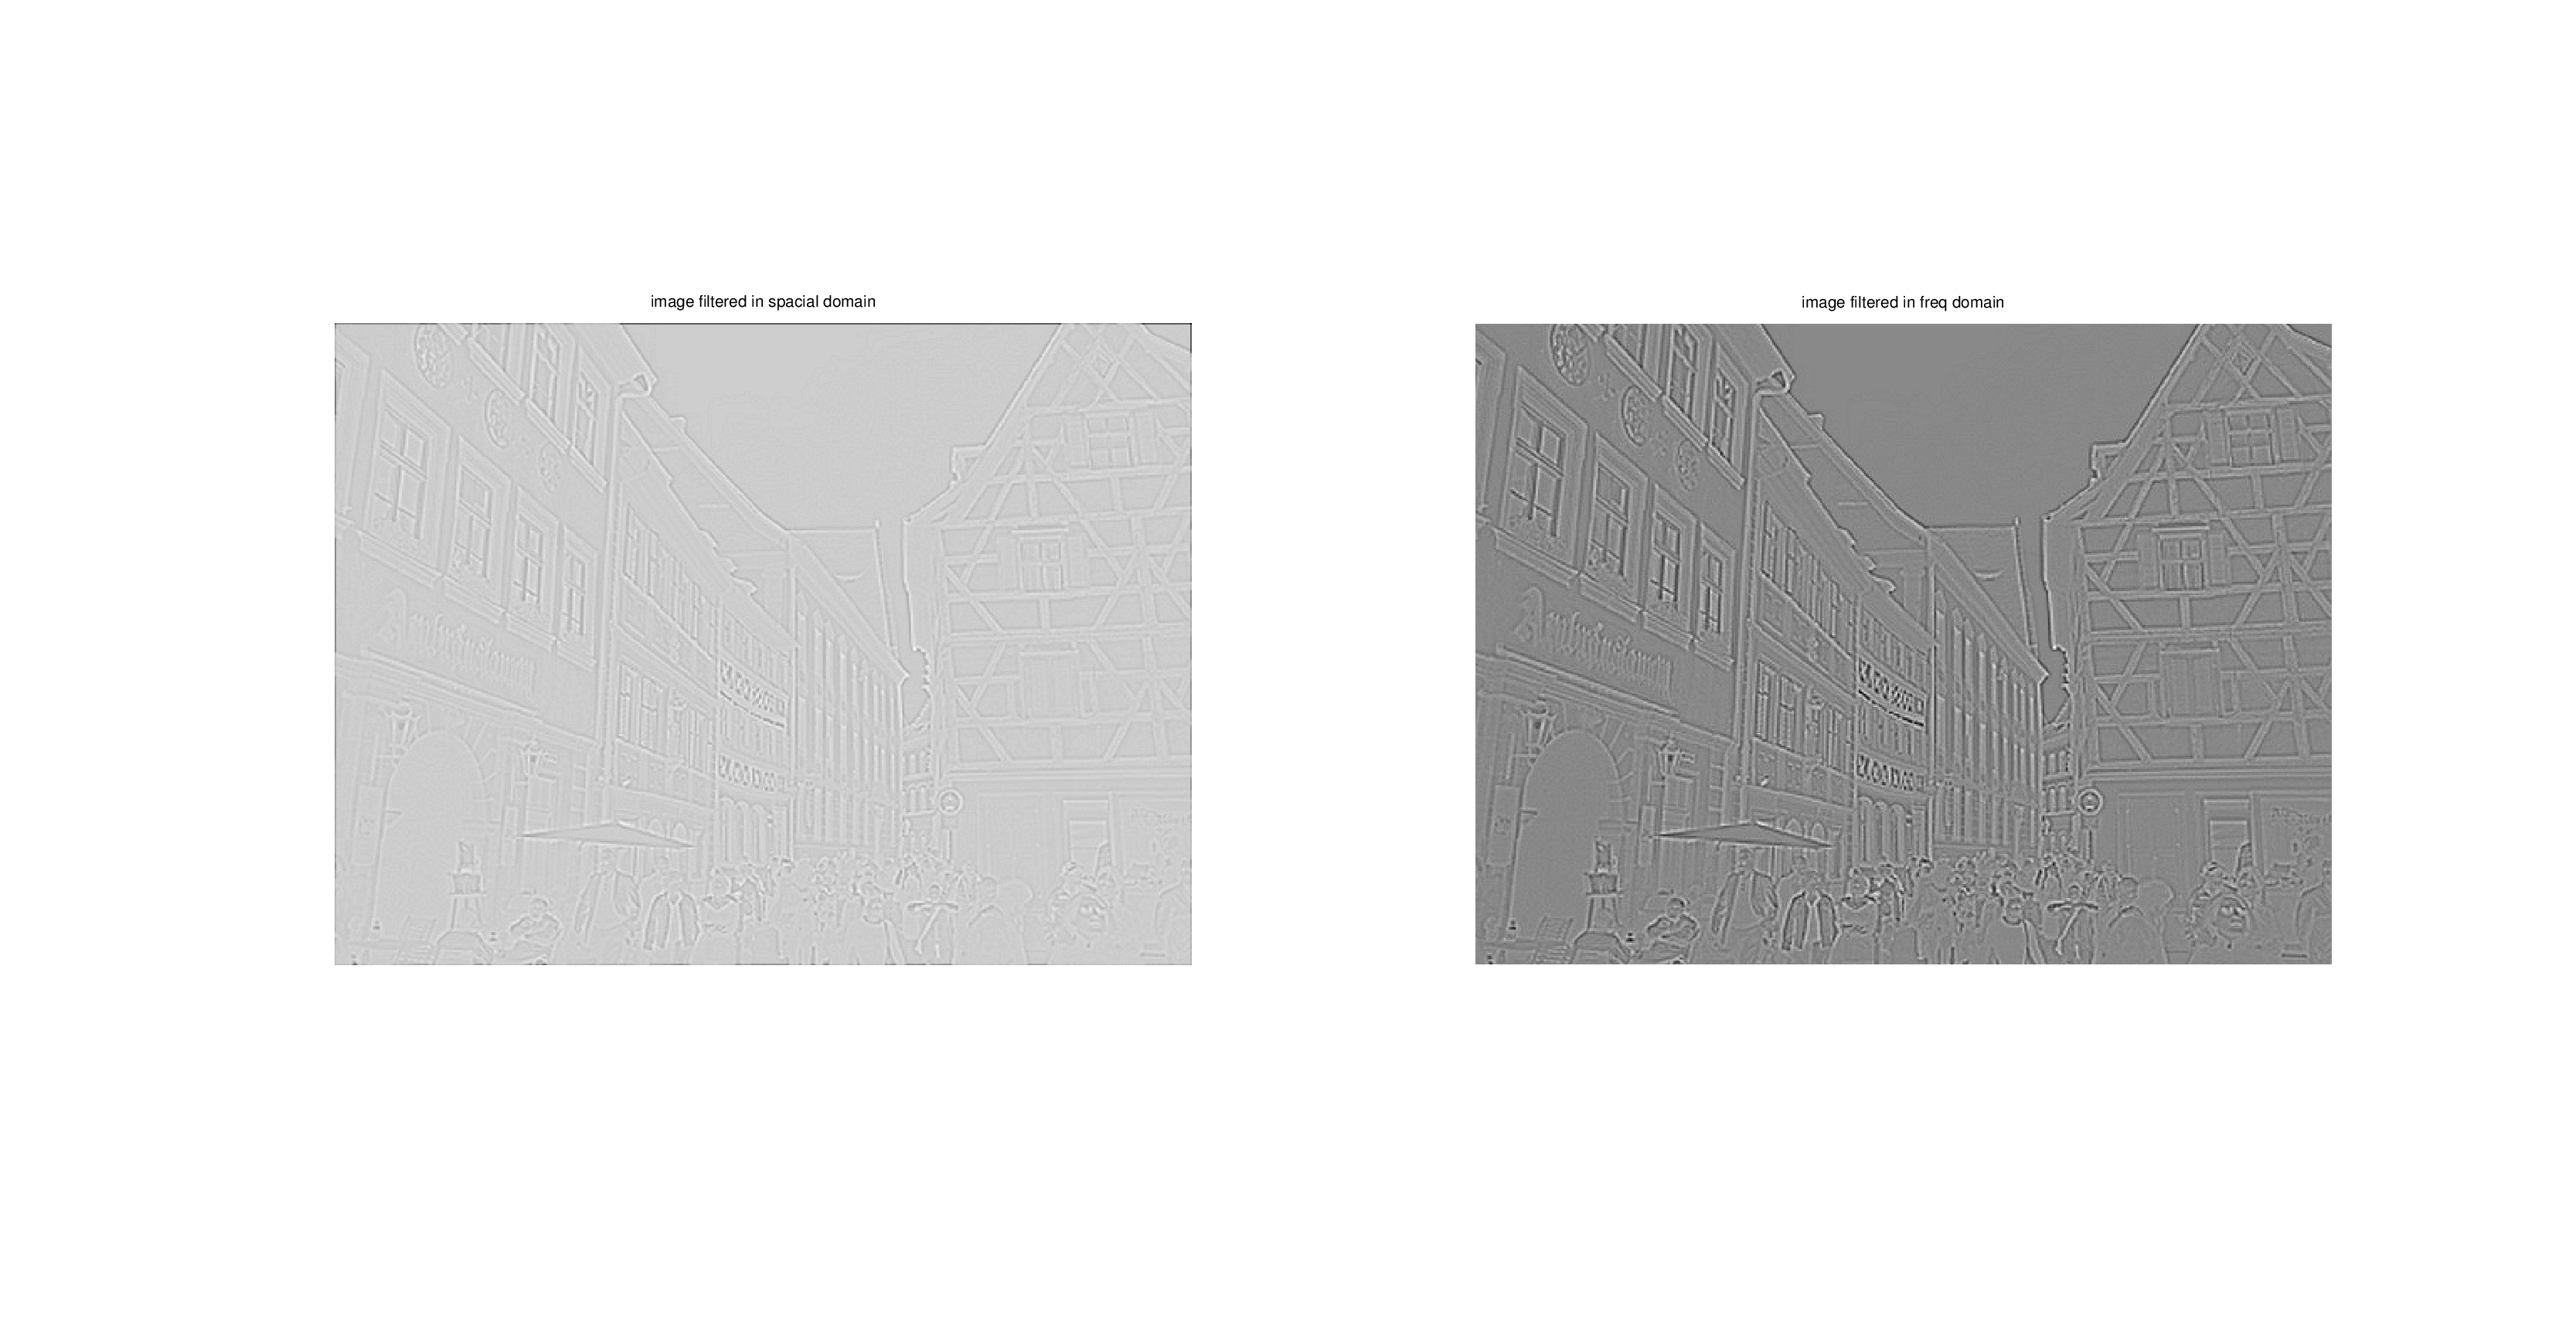
\includegraphics[width=\linewidth]{Q7/partC2.png}
		\caption{image filtered with laplacian filter}
	\end{figure}
	
	\begin{figure}[H]
		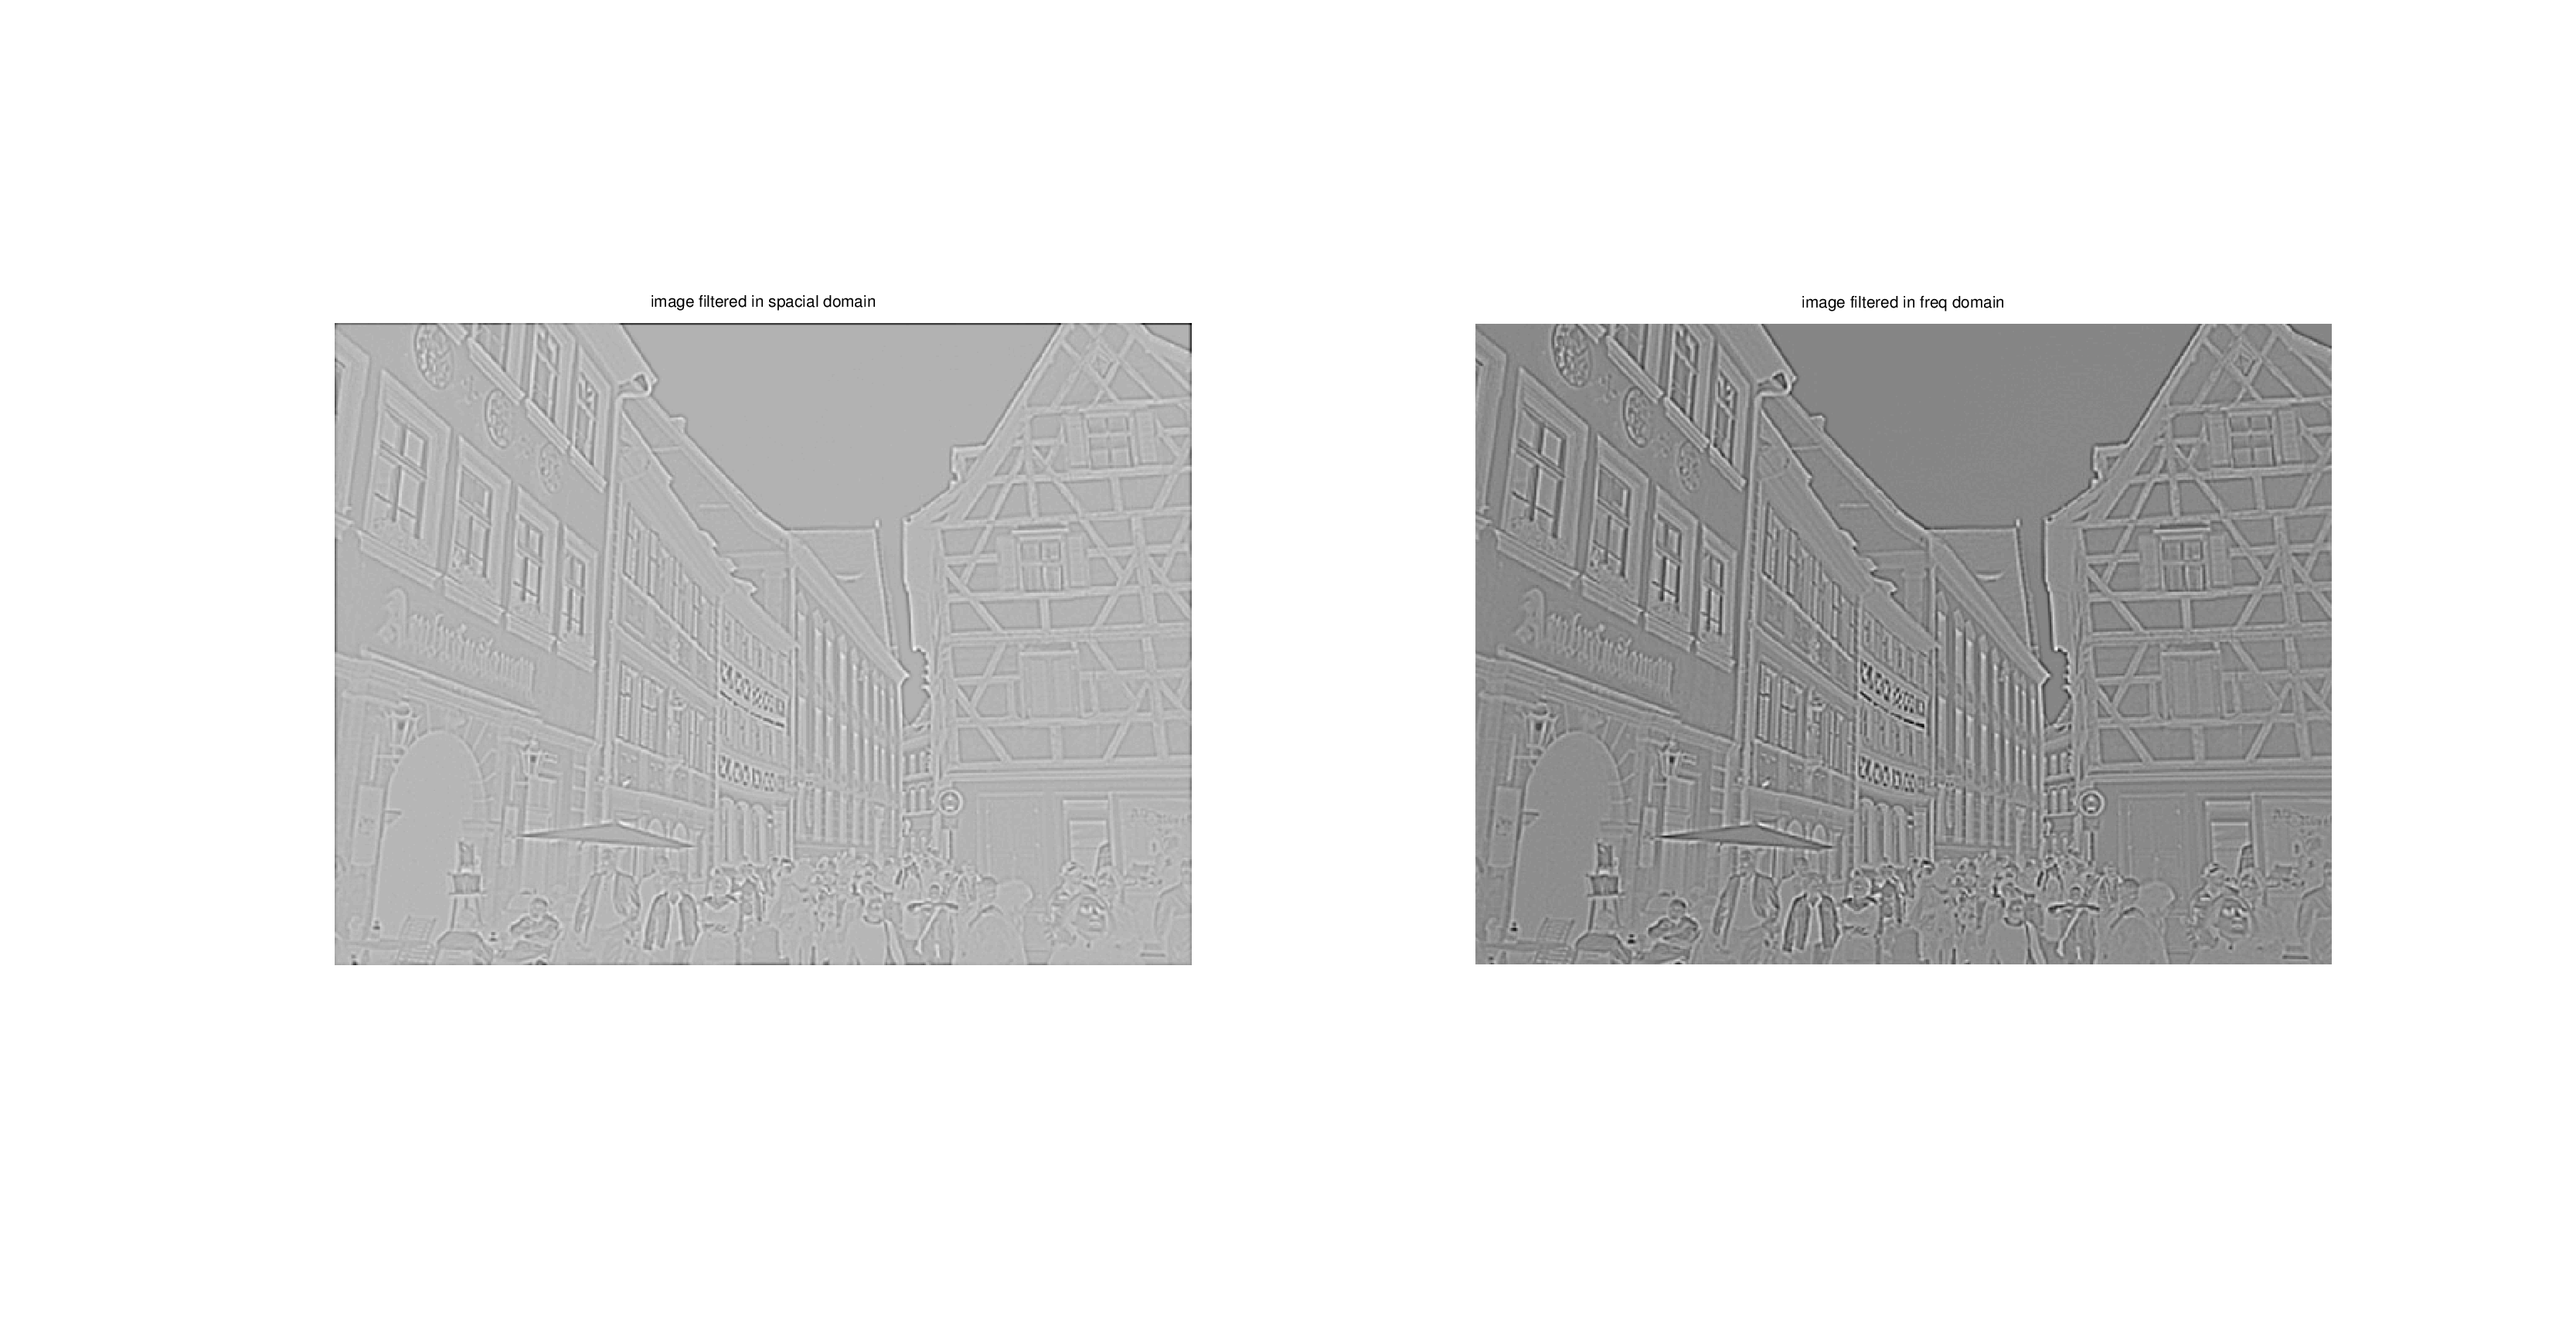
\includegraphics[width=\linewidth]{Q7/partC3.png}
		\caption{image filtered with LoG filter}
	\end{figure}
	
	There is a significant decrease of performance (25 to 40 times slower) when filtering in the frequency domain.
	\begin{table}[H]
		\centering
		\begin{tabular}{ c | c | c }
			filter & time for spacial dom & time for freq dom \\
			sobel & .006 & .169 \\
			laplacian & .006 & .223 \\
			LoG & .012 & .313 \\
		\end{tabular}
		\caption{time comparison for filtering in space vs freq domains}
	\end{table}
	
	\subsection{Ideal low pass and Gaussian}
	\begin{figure}[H]
		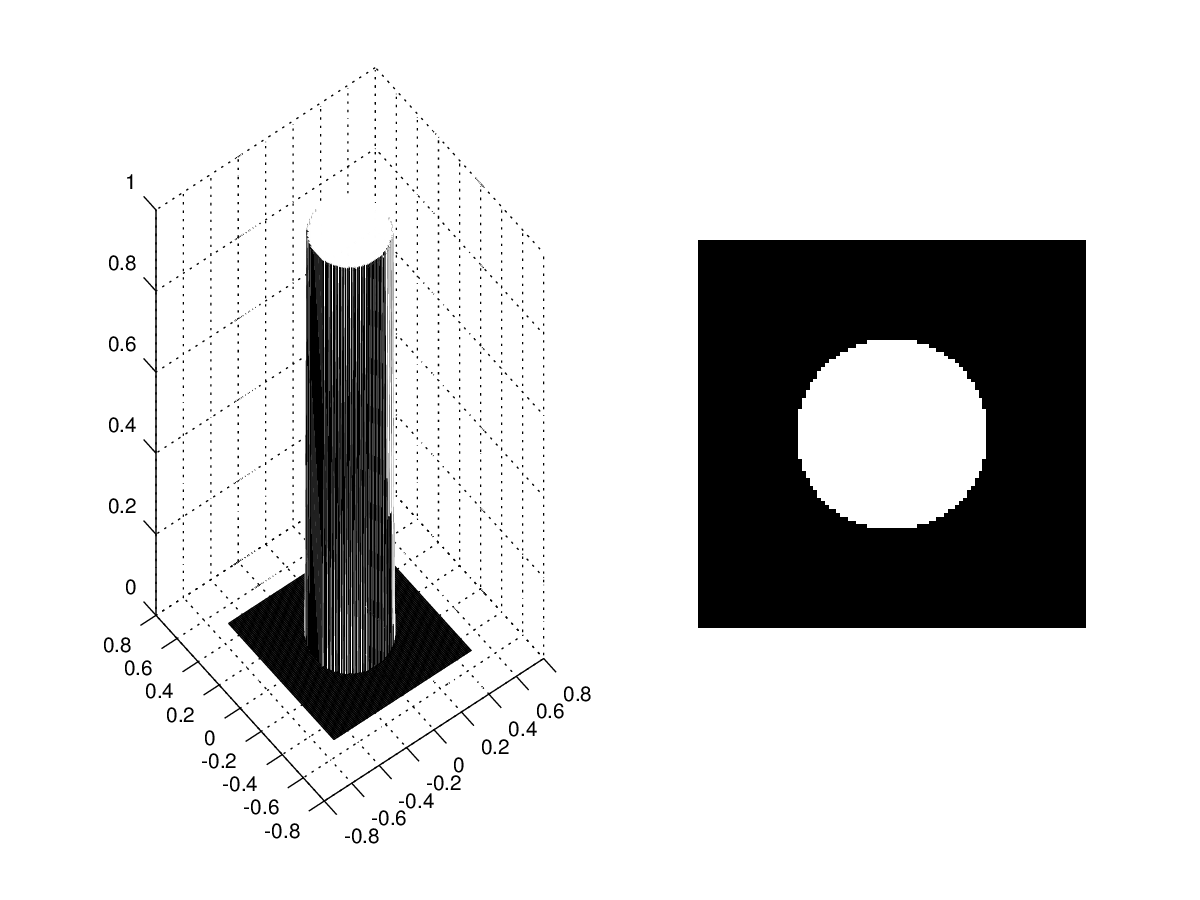
\includegraphics[width=\linewidth]{Q7/partD1.png}
		\caption{ideal low pass in freq domain}
	\end{figure}
	\begin{figure}[H]
		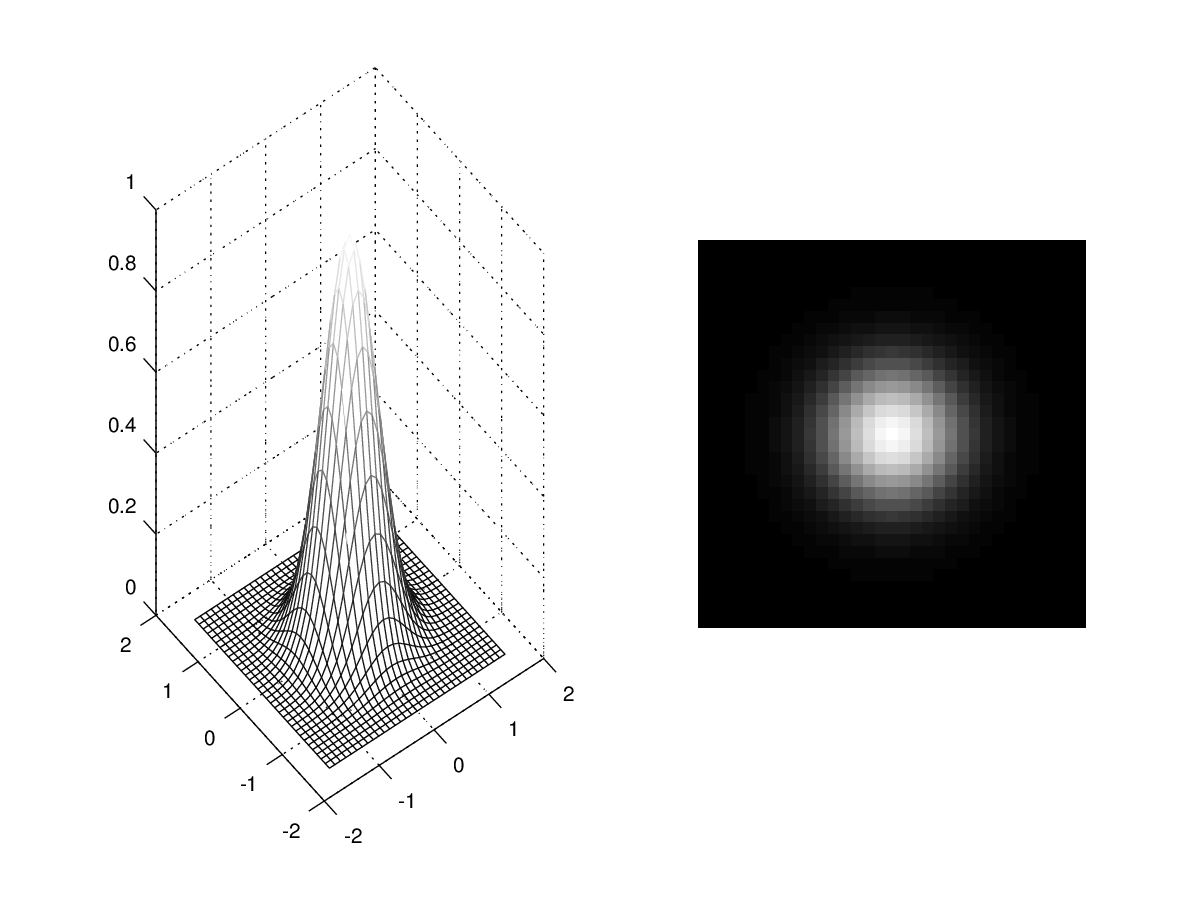
\includegraphics[width=\linewidth]{Q7/partD2.png}
		\caption{Gaussian filter with .4 sigma in freq domain}
	\end{figure}
	
	\subsection{Rectangular filter}
	\begin{figure}[H]
		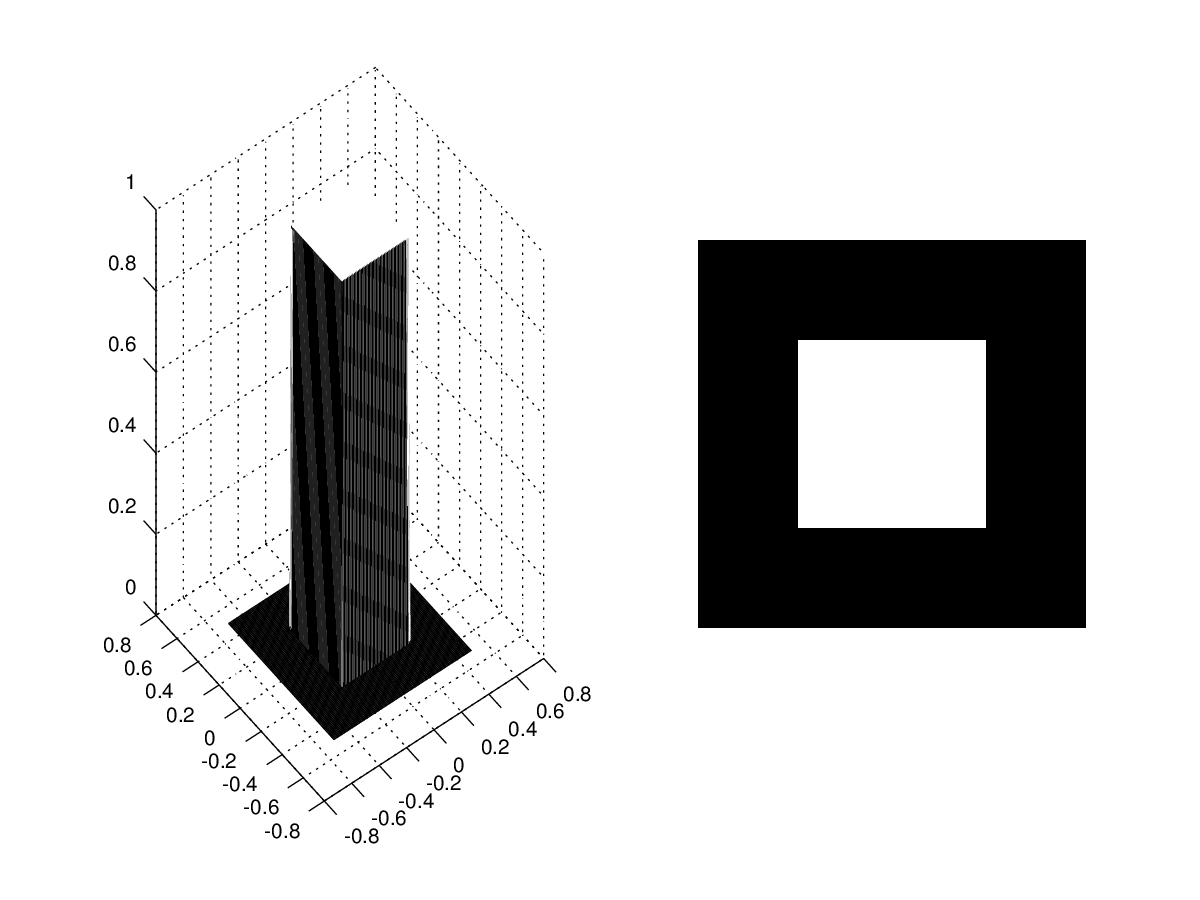
\includegraphics[width=\linewidth]{Q7/partE.png}
		\caption{rectangular filter in freq domain}
	\end{figure}
	
	\newpage
	\section{Code}
	\subsection{Q6}
	Code for smoothing
	\lstinputlisting[language=Octave]{Q6/partA.m}
	\newpage
	
	Code for sharpening
	\lstinputlisting[language=Octave]{Q6/partB.m}
	\newpage
	
	Utility Code
	\lstinputlisting[language=Octave]{Q6/normalizeImage.m}
	\newpage
	
	\subsection{Q7}
	Code to plot Fourier transform
	\lstinputlisting[language=Octave]{Q7/partA.m}
	\newpage
	
	Code for smoothing
	\lstinputlisting[language=Octave]{Q7/partB.m}
	\newpage
	
	Code for sharpening
	\lstinputlisting[language=Octave]{Q7/partC.m}
	
	\newpage
	Utility Code
	\lstinputlisting[language=Octave]{Q7/spaceAndFreqFilter.m}
	
	\newpage
	Code for plotting filters
	\lstinputlisting[language=Octave]{Q7/cylinderplot.m}
	\lstinputlisting[language=Octave]{Q7/gaussianplot.m}
	\lstinputlisting[language=Octave]{Q7/rectangleplot.m}
\end{document}
